\documentclass[12pt]{article}
\usepackage{commands}





\begin{document}









 \begin{tikzpicture}[remember picture,overlay]
         % If a chapter image has been specified
%         \expandafter\ifstrequal\expandafter{Images/vendingMachine.png}{}{}{
	                 % Output the chapter image
	                 \node[
	                 anchor=north west, % Anchor point on the image
	                 inner sep=0pt, % Inner padding
	                 ] at (current page.north west) {\includegraphics[angle=0,width=\paperwidth]{Images/Hilbert.jpg}};
%	         }
 \end{tikzpicture} 
 
  
  \vspace{-1.8cm}
\heading{Algebraic Properties of Hilbert Curve}


\newpage

\section*{Abstract}
I have came up with some interesting algebraic properties of the Hilbert curve which ultimately allows for an easy algorithm to generate the Hilbert curve of different orders, as well as studying the properties of this curve in higher levels of abstraction.


\section*{Methods}
Consider following pictorial elements which are the only elements needed to be combined to generate a Hilbert curve of any order.
\begin{figure}[h!]
	\centering
	
	
	
	\tikzset{every picture/.style={line width=0.75pt}} %set default line width to 0.75pt        
	
	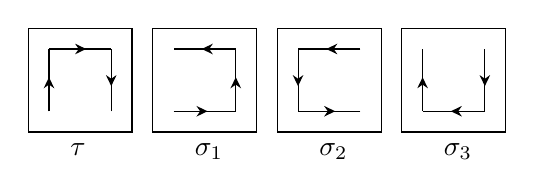
\begin{tikzpicture}[x=0.75pt,y=0.75pt,yscale=-1,xscale=1]
		%uncomment if require: \path (0,300); %set diagram left start at 0, and has height of 300
		
		%Shape: Square [id:dp8750923181633423] 
		\draw   (80,100) -- (130,100) -- (130,150) -- (80,150) -- cycle ;
		%Shape: Square [id:dp9461113500319673] 
		\draw   (140,100) -- (190,100) -- (190,150) -- (140,150) -- cycle ;
		%Shape: Square [id:dp0725116408752029] 
		\draw   (200,100) -- (250,100) -- (250,150) -- (200,150) -- cycle ;
		%Shape: Square [id:dp5827531683681308] 
		\draw   (260,100) -- (310,100) -- (310,150) -- (260,150) -- cycle ;
		%Straight Lines [id:da21981325377211292] 
		\draw    (90,140) -- (90,110) ;
		\draw [shift={(90,123.6)}, rotate = 90] [fill={rgb, 255:red, 0; green, 0; blue, 0 }  ][line width=0.08]  [draw opacity=0] (5.36,-2.57) -- (0,0) -- (5.36,2.57) -- (3.56,0) -- cycle    ;
		%Straight Lines [id:da10137471494621342] 
		\draw    (120,140) -- (120,110) ;
		\draw [shift={(120,127.9)}, rotate = 270] [fill={rgb, 255:red, 0; green, 0; blue, 0 }  ][line width=0.08]  [draw opacity=0] (5.36,-2.57) -- (0,0) -- (5.36,2.57) -- (3.56,0) -- cycle    ;
		%Straight Lines [id:da08669930636997147] 
		\draw    (120,110) -- (90,110) ;
		\draw [shift={(107.9,110)}, rotate = 180] [fill={rgb, 255:red, 0; green, 0; blue, 0 }  ][line width=0.08]  [draw opacity=0] (5.36,-2.57) -- (0,0) -- (5.36,2.57) -- (3.56,0) -- cycle    ;
		%Straight Lines [id:da8179506104727143] 
		\draw    (150,140) -- (180,140) ;
		\draw [shift={(166.4,140)}, rotate = 180] [fill={rgb, 255:red, 0; green, 0; blue, 0 }  ][line width=0.08]  [draw opacity=0] (5.36,-2.57) -- (0,0) -- (5.36,2.57) -- (3.56,0) -- cycle    ;
		%Straight Lines [id:da5631357790231875] 
		\draw    (180,140) -- (180,110) ;
		\draw [shift={(180,123.6)}, rotate = 90] [fill={rgb, 255:red, 0; green, 0; blue, 0 }  ][line width=0.08]  [draw opacity=0] (5.36,-2.57) -- (0,0) -- (5.36,2.57) -- (3.56,0) -- cycle    ;
		%Straight Lines [id:da2937680200727142] 
		\draw    (180,110) -- (150,110) ;
		\draw [shift={(163.6,110)}, rotate = 360] [fill={rgb, 255:red, 0; green, 0; blue, 0 }  ][line width=0.08]  [draw opacity=0] (5.36,-2.57) -- (0,0) -- (5.36,2.57) -- (3.56,0) -- cycle    ;
		%Straight Lines [id:da581952516784324] 
		\draw    (240,110) -- (210,110) ;
		\draw [shift={(223.6,110)}, rotate = 360] [fill={rgb, 255:red, 0; green, 0; blue, 0 }  ][line width=0.08]  [draw opacity=0] (5.36,-2.57) -- (0,0) -- (5.36,2.57) -- (3.56,0) -- cycle    ;
		%Straight Lines [id:da695850350935006] 
		\draw    (210,140) -- (210,110) ;
		\draw [shift={(210,127.9)}, rotate = 270] [fill={rgb, 255:red, 0; green, 0; blue, 0 }  ][line width=0.08]  [draw opacity=0] (5.36,-2.57) -- (0,0) -- (5.36,2.57) -- (3.56,0) -- cycle    ;
		%Straight Lines [id:da8929004198975072] 
		\draw    (240,140) -- (210,140) ;
		\draw [shift={(227.9,140)}, rotate = 180] [fill={rgb, 255:red, 0; green, 0; blue, 0 }  ][line width=0.08]  [draw opacity=0] (5.36,-2.57) -- (0,0) -- (5.36,2.57) -- (3.56,0) -- cycle    ;
		%Straight Lines [id:da6006060902326193] 
		\draw    (300,140) -- (300,110) ;
		\draw [shift={(300,127.9)}, rotate = 270] [fill={rgb, 255:red, 0; green, 0; blue, 0 }  ][line width=0.08]  [draw opacity=0] (5.36,-2.57) -- (0,0) -- (5.36,2.57) -- (3.56,0) -- cycle    ;
		%Straight Lines [id:da7922709761709981] 
		\draw    (300,140) -- (270,140) ;
		\draw [shift={(283.6,140)}, rotate = 360] [fill={rgb, 255:red, 0; green, 0; blue, 0 }  ][line width=0.08]  [draw opacity=0] (5.36,-2.57) -- (0,0) -- (5.36,2.57) -- (3.56,0) -- cycle    ;
		%Straight Lines [id:da9739097028731527] 
		\draw    (270,140) -- (270,110) ;
		\draw [shift={(270,123.6)}, rotate = 90] [fill={rgb, 255:red, 0; green, 0; blue, 0 }  ][line width=0.08]  [draw opacity=0] (5.36,-2.57) -- (0,0) -- (5.36,2.57) -- (3.56,0) -- cycle    ;
		
		% Text Node
		\draw (99,154.4) node [anchor=north west][inner sep=0.75pt]    {$\tau $};
		% Text Node
		\draw (159,154.4) node [anchor=north west][inner sep=0.75pt]    {$\sigma _{1}$};
		% Text Node
		\draw (219,154.4) node [anchor=north west][inner sep=0.75pt]    {$\sigma _{2}$};
		% Text Node
		\draw (279,154.4) node [anchor=north west][inner sep=0.75pt]    {$\sigma _{3}$};
		
		
	\end{tikzpicture}
\end{figure}
For instance, in the following figure we can see how these elements combined to give ruse to the whole structure.
\begin{figure}[h!]
	\centering
	
	
	
	\tikzset{every picture/.style={line width=0.75pt}} %set default line width to 0.75pt        
	
	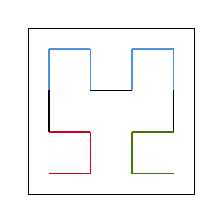
\begin{tikzpicture}[x=0.75pt,y=0.75pt,yscale=-1,xscale=1]
		%uncomment if require: \path (0,300); %set diagram left start at 0, and has height of 300
		
		%Straight Lines [id:da8407125579511403] 
		\draw [color={rgb, 255:red, 208; green, 2; blue, 27 }  ,draw opacity=1 ]   (90,170) -- (110,170) ;
		%Straight Lines [id:da9184250759282877] 
		\draw [color={rgb, 255:red, 208; green, 2; blue, 27 }  ,draw opacity=1 ]   (110,170) -- (110,150) ;
		%Straight Lines [id:da5127151604040254] 
		\draw [color={rgb, 255:red, 208; green, 2; blue, 27 }  ,draw opacity=1 ]   (110,150) -- (90,150) ;
		%Straight Lines [id:da9266164127300394] 
		\draw    (90,130) -- (90,150) ;
		%Straight Lines [id:da647108467210975] 
		\draw [color={rgb, 255:red, 74; green, 144; blue, 226 }  ,draw opacity=1 ]   (90,110) -- (90,130) ;
		%Straight Lines [id:da8751039194304964] 
		\draw [color={rgb, 255:red, 74; green, 144; blue, 226 }  ,draw opacity=1 ]   (110,110) -- (90,110) ;
		%Straight Lines [id:da94950575571884] 
		\draw [color={rgb, 255:red, 74; green, 144; blue, 226 }  ,draw opacity=1 ]   (110,130) -- (110,110) ;
		%Straight Lines [id:da13976027252025913] 
		\draw [color={rgb, 255:red, 74; green, 144; blue, 226 }  ,draw opacity=1 ]   (130,110) -- (130,130) ;
		%Straight Lines [id:da8414265169884174] 
		\draw [color={rgb, 255:red, 74; green, 144; blue, 226 }  ,draw opacity=1 ]   (150,110) -- (130,110) ;
		%Straight Lines [id:da7739455935113153] 
		\draw [color={rgb, 255:red, 74; green, 144; blue, 226 }  ,draw opacity=1 ]   (150,130) -- (150,110) ;
		%Straight Lines [id:da7529035264171824] 
		\draw    (110,130) -- (130,130) ;
		%Straight Lines [id:da28035376253282784] 
		\draw    (150,130) -- (150,150) ;
		%Straight Lines [id:da20674823733949532] 
		\draw [color={rgb, 255:red, 65; green, 117; blue, 5 }  ,draw opacity=1 ]   (150,150) -- (130,150) ;
		%Straight Lines [id:da722116120657142] 
		\draw [color={rgb, 255:red, 65; green, 117; blue, 5 }  ,draw opacity=1 ]   (130,170) -- (130,150) ;
		%Straight Lines [id:da7818847645191587] 
		\draw [color={rgb, 255:red, 65; green, 117; blue, 5 }  ,draw opacity=1 ]   (130,170) -- (150,170) ;
		%Shape: Square [id:dp45621549651067017] 
		\draw   (80,100) -- (160,100) -- (160,180) -- (80,180) -- cycle ;
		
		
		
		
	\end{tikzpicture}
\end{figure}
Although these elements are just pictorial elements, but thinking about them as permutations, we can then see their interactions with each other and if they interact nicely, we can construct the group structure out of these elements. 
\begin{figure}[h!]
	\centering
	
	
	
	\tikzset{every picture/.style={line width=0.75pt}} %set default line width to 0.75pt        
	
	\begin{tikzpicture}[x=0.75pt,y=0.75pt,yscale=-1,xscale=1]
		%uncomment if require: \path (0,300); %set diagram left start at 0, and has height of 300
		
		%Shape: Square [id:dp8656559393447294] 
		\draw  [color={rgb, 255:red, 155; green, 155; blue, 155 }  ,draw opacity=1 ][dash pattern={on 4.5pt off 4.5pt}] (100,30) -- (140,30) -- (140,70) -- (100,70) -- cycle ;
		%Shape: Square [id:dp25819654894625055] 
		\draw  [color={rgb, 255:red, 155; green, 155; blue, 155 }  ,draw opacity=1 ][dash pattern={on 4.5pt off 4.5pt}] (60,70) -- (100,70) -- (100,110) -- (60,110) -- cycle ;
		%Shape: Square [id:dp12855032985022108] 
		\draw  [color={rgb, 255:red, 128; green, 128; blue, 128 }  ,draw opacity=1 ] (60,30) -- (140,30) -- (140,110) -- (60,110) -- cycle ;
		%Straight Lines [id:da46762945679293644] 
		\draw    (80,90) -- (80,50) ;
		\draw [shift={(80,68.6)}, rotate = 90] [fill={rgb, 255:red, 0; green, 0; blue, 0 }  ][line width=0.08]  [draw opacity=0] (5.36,-2.57) -- (0,0) -- (5.36,2.57) -- (3.56,0) -- cycle    ;
		%Straight Lines [id:da19491668085227998] 
		\draw    (80,50) -- (120,50) ;
		\draw [shift={(101.4,50)}, rotate = 180] [fill={rgb, 255:red, 0; green, 0; blue, 0 }  ][line width=0.08]  [draw opacity=0] (5.36,-2.57) -- (0,0) -- (5.36,2.57) -- (3.56,0) -- cycle    ;
		%Straight Lines [id:da5946725269414244] 
		\draw    (120,50) -- (120,90) ;
		\draw [shift={(120,71.4)}, rotate = 270] [fill={rgb, 255:red, 0; green, 0; blue, 0 }  ][line width=0.08]  [draw opacity=0] (5.36,-2.57) -- (0,0) -- (5.36,2.57) -- (3.56,0) -- cycle    ;
		%Shape: Square [id:dp40814238067266806] 
		\draw  [color={rgb, 255:red, 155; green, 155; blue, 155 }  ,draw opacity=1 ][dash pattern={on 4.5pt off 4.5pt}] (240,30) -- (280,30) -- (280,70) -- (240,70) -- cycle ;
		%Shape: Square [id:dp3190214011077266] 
		\draw  [color={rgb, 255:red, 155; green, 155; blue, 155 }  ,draw opacity=1 ][dash pattern={on 4.5pt off 4.5pt}] (200,70) -- (240,70) -- (240,110) -- (200,110) -- cycle ;
		%Shape: Square [id:dp020521430574480082] 
		\draw  [color={rgb, 255:red, 128; green, 128; blue, 128 }  ,draw opacity=1 ] (200,30) -- (280,30) -- (280,110) -- (200,110) -- cycle ;
		%Straight Lines [id:da5681454863412756] 
		\draw    (220,90) -- (260,90) ;
		\draw [shift={(241.4,90)}, rotate = 180] [fill={rgb, 255:red, 0; green, 0; blue, 0 }  ][line width=0.08]  [draw opacity=0] (5.36,-2.57) -- (0,0) -- (5.36,2.57) -- (3.56,0) -- cycle    ;
		%Straight Lines [id:da9020319519818625] 
		\draw    (260,50) -- (220,50) ;
		\draw [shift={(238.6,50)}, rotate = 360] [fill={rgb, 255:red, 0; green, 0; blue, 0 }  ][line width=0.08]  [draw opacity=0] (5.36,-2.57) -- (0,0) -- (5.36,2.57) -- (3.56,0) -- cycle    ;
		%Straight Lines [id:da3531240438970169] 
		\draw    (260,90) -- (260,50) ;
		\draw [shift={(260,68.6)}, rotate = 90] [fill={rgb, 255:red, 0; green, 0; blue, 0 }  ][line width=0.08]  [draw opacity=0] (5.36,-2.57) -- (0,0) -- (5.36,2.57) -- (3.56,0) -- cycle    ;
		%Shape: Square [id:dp572853131688938] 
		\draw  [color={rgb, 255:red, 155; green, 155; blue, 155 }  ,draw opacity=1 ][dash pattern={on 4.5pt off 4.5pt}] (520,30) -- (560,30) -- (560,70) -- (520,70) -- cycle ;
		%Shape: Square [id:dp9499933922676527] 
		\draw  [color={rgb, 255:red, 155; green, 155; blue, 155 }  ,draw opacity=1 ][dash pattern={on 4.5pt off 4.5pt}] (480,70) -- (520,70) -- (520,110) -- (480,110) -- cycle ;
		%Shape: Square [id:dp4671101672592797] 
		\draw  [color={rgb, 255:red, 128; green, 128; blue, 128 }  ,draw opacity=1 ] (480,30) -- (560,30) -- (560,110) -- (480,110) -- cycle ;
		%Straight Lines [id:da0909155103730872] 
		\draw    (540,90) -- (500,90) ;
		\draw [shift={(518.6,90)}, rotate = 360] [fill={rgb, 255:red, 0; green, 0; blue, 0 }  ][line width=0.08]  [draw opacity=0] (5.36,-2.57) -- (0,0) -- (5.36,2.57) -- (3.56,0) -- cycle    ;
		%Straight Lines [id:da4754650711157731] 
		\draw    (540,50) -- (540,90) ;
		\draw [shift={(540,71.4)}, rotate = 270] [fill={rgb, 255:red, 0; green, 0; blue, 0 }  ][line width=0.08]  [draw opacity=0] (5.36,-2.57) -- (0,0) -- (5.36,2.57) -- (3.56,0) -- cycle    ;
		%Straight Lines [id:da7292234694186692] 
		\draw    (500,90) -- (500,50) ;
		\draw [shift={(500,68.6)}, rotate = 90] [fill={rgb, 255:red, 0; green, 0; blue, 0 }  ][line width=0.08]  [draw opacity=0] (5.36,-2.57) -- (0,0) -- (5.36,2.57) -- (3.56,0) -- cycle    ;
		%Shape: Square [id:dp05552233392147787] 
		\draw  [color={rgb, 255:red, 155; green, 155; blue, 155 }  ,draw opacity=1 ][dash pattern={on 4.5pt off 4.5pt}] (380,30) -- (420,30) -- (420,70) -- (380,70) -- cycle ;
		%Shape: Square [id:dp2954745205845595] 
		\draw  [color={rgb, 255:red, 155; green, 155; blue, 155 }  ,draw opacity=1 ][dash pattern={on 4.5pt off 4.5pt}] (340,70) -- (380,70) -- (380,110) -- (340,110) -- cycle ;
		%Shape: Square [id:dp09171668575457348] 
		\draw  [color={rgb, 255:red, 128; green, 128; blue, 128 }  ,draw opacity=1 ] (340,30) -- (420,30) -- (420,110) -- (340,110) -- cycle ;
		%Straight Lines [id:da503613097684924] 
		\draw    (360,90) -- (400,90) ;
		\draw [shift={(381.4,90)}, rotate = 180] [fill={rgb, 255:red, 0; green, 0; blue, 0 }  ][line width=0.08]  [draw opacity=0] (5.36,-2.57) -- (0,0) -- (5.36,2.57) -- (3.56,0) -- cycle    ;
		%Straight Lines [id:da2263819791298236] 
		\draw    (400,50) -- (360,50) ;
		\draw [shift={(378.6,50)}, rotate = 360] [fill={rgb, 255:red, 0; green, 0; blue, 0 }  ][line width=0.08]  [draw opacity=0] (5.36,-2.57) -- (0,0) -- (5.36,2.57) -- (3.56,0) -- cycle    ;
		%Straight Lines [id:da4223916331418833] 
		\draw    (360,90) -- (360,50) ;
		\draw [shift={(360,68.6)}, rotate = 90] [fill={rgb, 255:red, 0; green, 0; blue, 0 }  ][line width=0.08]  [draw opacity=0] (5.36,-2.57) -- (0,0) -- (5.36,2.57) -- (3.56,0) -- cycle    ;
		
		% Text Node
		\draw (61,102.4) node [anchor=north west][inner sep=0.75pt]  [font=\tiny,color={rgb, 255:red, 128; green, 128; blue, 128 }  ,opacity=1 ]  {$0$};
		% Text Node
		\draw (61,62.4) node [anchor=north west][inner sep=0.75pt]  [font=\tiny,color={rgb, 255:red, 128; green, 128; blue, 128 }  ,opacity=1 ]  {$1$};
		% Text Node
		\draw (101,62.4) node [anchor=north west][inner sep=0.75pt]  [font=\tiny,color={rgb, 255:red, 128; green, 128; blue, 128 }  ,opacity=1 ]  {$2$};
		% Text Node
		\draw (101,102.4) node [anchor=north west][inner sep=0.75pt]  [font=\tiny,color={rgb, 255:red, 128; green, 128; blue, 128 }  ,opacity=1 ]  {$3$};
		% Text Node
		\draw (43,132.4) node [anchor=north west][inner sep=0.75pt]  [font=\footnotesize]  {$\tau =\begin{pmatrix}
				0 & 1 & 2 & 3\\
				0 & 1 & 2 & 3
			\end{pmatrix}$};
		% Text Node
		\draw (201,102.4) node [anchor=north west][inner sep=0.75pt]  [font=\tiny,color={rgb, 255:red, 128; green, 128; blue, 128 }  ,opacity=1 ]  {$0$};
		% Text Node
		\draw (241,102.4) node [anchor=north west][inner sep=0.75pt]  [font=\tiny,color={rgb, 255:red, 128; green, 128; blue, 128 }  ,opacity=1 ]  {$1$};
		% Text Node
		\draw (241,62.4) node [anchor=north west][inner sep=0.75pt]  [font=\tiny,color={rgb, 255:red, 128; green, 128; blue, 128 }  ,opacity=1 ]  {$2$};
		% Text Node
		\draw (201,62.4) node [anchor=north west][inner sep=0.75pt]  [font=\tiny,color={rgb, 255:red, 128; green, 128; blue, 128 }  ,opacity=1 ]  {$3$};
		% Text Node
		\draw (176,132.4) node [anchor=north west][inner sep=0.75pt]  [font=\footnotesize]  {$\sigma _{1} =\begin{pmatrix}
				0 & 1 & 2 & 3\\
				0 & 3 & 2 & 1
			\end{pmatrix}$};
		% Text Node
		\draw (521,62.4) node [anchor=north west][inner sep=0.75pt]  [font=\tiny,color={rgb, 255:red, 128; green, 128; blue, 128 }  ,opacity=1 ]  {$0$};
		% Text Node
		\draw (521,102.4) node [anchor=north west][inner sep=0.75pt]  [font=\tiny,color={rgb, 255:red, 128; green, 128; blue, 128 }  ,opacity=1 ]  {$1$};
		% Text Node
		\draw (481,102.4) node [anchor=north west][inner sep=0.75pt]  [font=\tiny,color={rgb, 255:red, 128; green, 128; blue, 128 }  ,opacity=1 ]  {$2$};
		% Text Node
		\draw (481,62.4) node [anchor=north west][inner sep=0.75pt]  [font=\tiny,color={rgb, 255:red, 128; green, 128; blue, 128 }  ,opacity=1 ]  {$3$};
		% Text Node
		\draw (317,132.4) node [anchor=north west][inner sep=0.75pt]  [font=\footnotesize]  {$\sigma _{2} =\begin{pmatrix}
				0 & 1 & 2 & 3\\
				2 & 1 & 0 & 3
			\end{pmatrix}$};
		% Text Node
		\draw (381,62.4) node [anchor=north west][inner sep=0.75pt]  [font=\tiny,color={rgb, 255:red, 128; green, 128; blue, 128 }  ,opacity=1 ]  {$0$};
		% Text Node
		\draw (341,62.4) node [anchor=north west][inner sep=0.75pt]  [font=\tiny,color={rgb, 255:red, 128; green, 128; blue, 128 }  ,opacity=1 ]  {$1$};
		% Text Node
		\draw (341,102.4) node [anchor=north west][inner sep=0.75pt]  [font=\tiny,color={rgb, 255:red, 128; green, 128; blue, 128 }  ,opacity=1 ]  {$2$};
		% Text Node
		\draw (381,102.4) node [anchor=north west][inner sep=0.75pt]  [font=\tiny,color={rgb, 255:red, 128; green, 128; blue, 128 }  ,opacity=1 ]  {$3$};
		% Text Node
		\draw (457,132.4) node [anchor=north west][inner sep=0.75pt]  [font=\footnotesize]  {$\sigma _{3} =\begin{pmatrix}
				0 & 1 & 2 & 3\\
				2 & 3 & 0 & 1
			\end{pmatrix}$};
		
		
	\end{tikzpicture}
\end{figure}

\begin{theorem}
	\label{thm:GIsGroup}
	Consider the set $ G = \set{\tau, \sigma_1, \sigma_2, \sigma_3} $. Then $ (G,\circ) $ has a group structure where $ \circ $ is the composition of functions form a group.
\end{theorem}
\begin{proof}
	This follows immediately by calculating the elements of the following product table
	\begin{center}
			\begin{tabular}{c|cccc}
			& $\tau$ & $\sigma_1$ & $\sigma_2$ & $\sigma_3$ \\
			\hline
			$\tau$ & $\tau$ & $\sigma_1$ & $\sigma_2$ & $\sigma_3$ \\
			$\sigma_1$ & $\sigma_1$ & $\tau$ & $\sigma_3$ & $\sigma_2$ \\
			$\sigma_2$ & $\sigma_2$ & $\sigma_3$ & $\tau$ & $\sigma_1$ \\
			$\sigma_3$ & $\sigma_3$ & $\sigma_2$ & $\sigma_1$ & $\tau$ \\
		\end{tabular}
	\end{center}
	Since the product table above is symmetric, then it follows that this group is an Abelian group as well. This completes the proof.
\end{proof}



\begin{remark}
	For a more clean notation, we write $ ab $ instead of $ a\circ b $ where $ a $ and $ b $ are the elements of group.
\end{remark}

\subsection*{First Algebraic Construction of the Hilbert Curve}
In the product table calculated in \autoref{thm:GIsGroup} we know how the elements of the group interact with each other. However, for the first algebraic construction of the Hilbert curve we also need to define how the group $ G $ acts on matrices.
\begin{definition}[Right action of group $ G $ on matrices]
	\label{def:RightactionOFgroup}
	Let $ M $ be a $2\times 2$ matrix whose elements are from the set $ G $ as in \autoref{thm:GIsGroup}. Then the right action of group $ G $ on $ M $ is defined to be
	\begin{align*}
		\tau \matt{a}{b}{c}{d} &= \matt{a}{b}{c}{d},\\
		\sigma_1 \matt{a}{b}{c}{d} &= \matt{\sigma_1a}{\sigma_1b}{\sigma_1c}{\sigma_1d}^{[\sigma_1]} = \matt{\sigma_1 d}{\sigma_1 b}{\sigma_1 c}{\sigma_1 a},\\
		\sigma_2 \matt{a}{b}{c}{d} &= \matt{\sigma_2a}{\sigma_2b}{\sigma_2c}{\sigma_2d}^{[\sigma_2]} = \matt{\sigma_2 a}{\sigma_2 c}{\sigma_2 b}{\sigma_2 d},\\
		\sigma_3 \matt{a}{b}{c}{d} &= \matt{\sigma_3a}{\sigma_3b}{\sigma_3c}{\sigma_3d}^{[\sigma_3]} = \matt{\sigma_2 d}{\sigma_2 c}{\sigma_2 b}{\sigma_2 a}.\\
	\end{align*}
	Similarly, for $ \tilde{M} $ a $ 2^{d+1}\times 2^{d+1} $ matrix action of any $ \omega \in G $ on $ \tilde{M} $ is defined to be
	\[ \omega \tilde{M} = \omega \matt{A}{B}{C}{D} = \matt{\omega A}{\omega B}{\omega C}{\omega D}^{[\omega ]}\]
\end{definition}

\begin{construction}(Iterative Construction of Hilbert Curve)
	Define the map 
	\[  F_n : G^{2^n}\times G^{2^n} \to G^{2^{n+1}}\times G^{2^{n+1}}  \]
	give as 
	\begin{figure}[h!]
	\centering 
	
	


\tikzset{every picture/.style={line width=0.75pt}} %set default line width to 0.75pt        

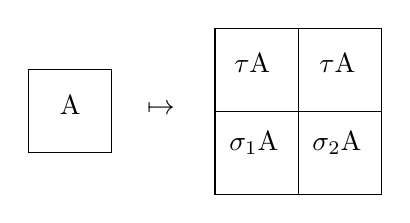
\begin{tikzpicture}[x=0.75pt,y=0.75pt,yscale=-1,xscale=1]
	%uncomment if require: \path (0,300); %set diagram left start at 0, and has height of 300
	
	%Shape: Square [id:dp2023056445996656] 
	\draw   (80,130) -- (120,130) -- (120,170) -- (80,170) -- cycle ;
	%Shape: Square [id:dp7368055726038727] 
	\draw   (170,110) -- (210,110) -- (210,150) -- (170,150) -- cycle ;
	%Shape: Square [id:dp2426334503608445] 
	\draw   (170,150) -- (210,150) -- (210,190) -- (170,190) -- cycle ;
	%Shape: Square [id:dp48040422500928703] 
	\draw   (210,110) -- (250,110) -- (250,150) -- (210,150) -- cycle ;
	%Shape: Square [id:dp2369707217947341] 
	\draw   (210,150) -- (250,150) -- (250,190) -- (210,190) -- cycle ;
	
	% Text Node
	\draw (175.67,158.67) node [anchor=north west][inner sep=0.75pt]   [align=left] {$\displaystyle \sigma _{1}$A};
	% Text Node
	\draw (215.67,158.67) node [anchor=north west][inner sep=0.75pt]   [align=left] {$\displaystyle \sigma _{2}$A};
	% Text Node
	\draw (94,141) node [anchor=north west][inner sep=0.75pt]   [align=left] {A};
	% Text Node
	\draw (136,145.4) node [anchor=north west][inner sep=0.75pt]    {$\mapsto $};
	% Text Node
	\draw (178,121) node [anchor=north west][inner sep=0.75pt]   [align=left] {$\displaystyle \tau $A};
	% Text Node
	\draw (219,121) node [anchor=north west][inner sep=0.75pt]   [align=left] {$\displaystyle \tau $A};
	
	
\end{tikzpicture}
\end{figure}
	\FloatBarrier
	Applying this map iteratively on $ 1\times 1 $ matrix $ \begin{bmatrix}  \tau  \end{bmatrix} $ for $ n $ times will generate the Hilbert curve of degree $ n $. 
\end{construction}
For instance, this construction predicts that the overall shape of the 4-th order Hilbert curve will be
\[ 
\boxed{\begin{array}{cccccccc}
	\tau & \tau & \tau & \tau & \tau & \tau & \tau & \tau \\
	\sigma_1 & \sigma_2 & \sigma_1 & \sigma_2 & \sigma_1 & \sigma_2 & \sigma_1 & \sigma_2 \\
	\sigma_3 & \sigma_1 & \sigma_2 & \sigma_3 & \sigma_3 & \sigma_1 & \sigma_2 & \sigma_3 \\
	\tau & \sigma_1 & \sigma_2 & \tau & \tau & \sigma_1 & \sigma_2 & \tau \\
	\sigma_1 & \sigma_2 & \sigma_3 & \sigma_1 & \sigma_2 & \sigma_3 & \sigma_1 & \sigma_2 \\
	\sigma_3 & \sigma_3 & \tau & \sigma_1 & \sigma_2 & \tau & \sigma_3 & \sigma_3 \\
	\tau & \tau & \sigma_3 & \sigma_1 & \sigma_2 & \sigma_3 & \tau & \tau \\
	\sigma_1 & \sigma_2 & \tau & \sigma_1 & \sigma_2 & \tau & \sigma_1 & \sigma_2
\end{array}}
\]


\subsection*{Second Algebraic Construction of the Hilbert Curve}
This method is easier to implement in a computer. Equivalent to \autoref{def:RightactionOFgroup} we can think of acting a permutation on a matrix of permutations as 
\begin{figure}[h!]
	\centering
	
	
	\tikzset{every picture/.style={line width=0.75pt}} %set default line width to 0.75pt        
	
	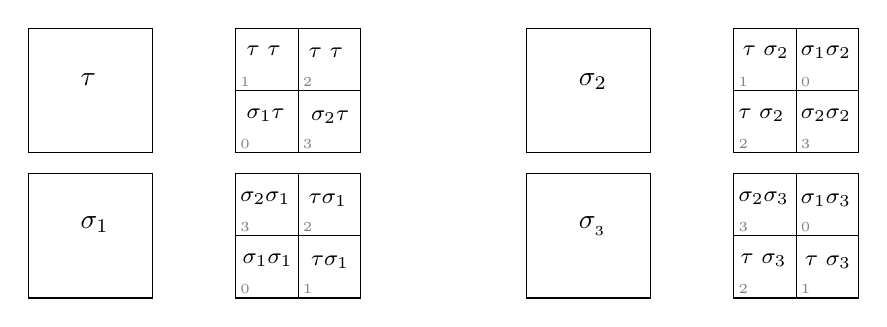
\begin{tikzpicture}[x=0.75pt,y=0.75pt,yscale=-1,xscale=1]
		%uncomment if require: \path (0,300); %set diagram left start at 0, and has height of 300
		
		%Shape: Square [id:dp5131155499816018] 
		\draw   (100,10) -- (160,10) -- (160,70) -- (100,70) -- cycle ;
		%Shape: Square [id:dp32281460324226097] 
		\draw   (200,10) -- (260,10) -- (260,70) -- (200,70) -- cycle ;
		%Shape: Square [id:dp8196638610158489] 
		\draw   (200,40) -- (230,40) -- (230,70) -- (200,70) -- cycle ;
		%Shape: Square [id:dp5774035572053016] 
		\draw   (230,10) -- (260,10) -- (260,40) -- (230,40) -- cycle ;
		%Shape: Square [id:dp4820583847814002] 
		\draw   (100,80) -- (160,80) -- (160,140) -- (100,140) -- cycle ;
		%Shape: Square [id:dp9404167053590688] 
		\draw   (200,80) -- (260,80) -- (260,140) -- (200,140) -- cycle ;
		%Shape: Square [id:dp9877852027747471] 
		\draw   (200,110) -- (230,110) -- (230,140) -- (200,140) -- cycle ;
		%Shape: Square [id:dp7983426749714371] 
		\draw   (230,80) -- (260,80) -- (260,110) -- (230,110) -- cycle ;
		%Shape: Square [id:dp9838717655019427] 
		\draw   (340,10) -- (400,10) -- (400,70) -- (340,70) -- cycle ;
		%Shape: Square [id:dp20385470609057088] 
		\draw   (440,10) -- (500,10) -- (500,70) -- (440,70) -- cycle ;
		%Shape: Square [id:dp48605235834359806] 
		\draw   (440,40) -- (470,40) -- (470,70) -- (440,70) -- cycle ;
		%Shape: Square [id:dp45051660905134305] 
		\draw   (470,10) -- (500,10) -- (500,40) -- (470,40) -- cycle ;
		%Shape: Square [id:dp8452440310958111] 
		\draw   (340,80) -- (400,80) -- (400,140) -- (340,140) -- cycle ;
		%Shape: Square [id:dp6874281190393423] 
		\draw   (440,80) -- (500,80) -- (500,140) -- (440,140) -- cycle ;
		%Shape: Square [id:dp3947498884896019] 
		\draw   (440,110) -- (470,110) -- (470,140) -- (440,140) -- cycle ;
		%Shape: Square [id:dp7927640676642602] 
		\draw   (470,80) -- (500,80) -- (500,110) -- (470,110) -- cycle ;
		
		% Text Node
		\draw (124,30.4) node [anchor=north west][inner sep=0.75pt]    {$\tau $};
		% Text Node
		\draw (204,47.4) node [anchor=north west][inner sep=0.75pt]  [font=\footnotesize]  {$\sigma_{1} \tau $};
		% Text Node
		\draw (204,17.4) node [anchor=north west][inner sep=0.75pt]  [font=\footnotesize]  {$\tau \ \tau $};
		% Text Node
		\draw (234,18.4) node [anchor=north west][inner sep=0.75pt]  [font=\footnotesize]  {$\tau \ \tau $};
		% Text Node
		\draw (235,48.4) node [anchor=north west][inner sep=0.75pt]  [font=\footnotesize]  {$\sigma_{2} \tau $};
		% Text Node
		\draw (201,62.4) node [anchor=north west][inner sep=0.75pt]  [font=\tiny,color={rgb, 255:red, 128; green, 128; blue, 128 }  ,opacity=1 ]  {$0$};
		% Text Node
		\draw (201,32.4) node [anchor=north west][inner sep=0.75pt]  [font=\tiny,color={rgb, 255:red, 128; green, 128; blue, 128 }  ,opacity=1 ]  {$1$};
		% Text Node
		\draw (231,32.4) node [anchor=north west][inner sep=0.75pt]  [font=\tiny,color={rgb, 255:red, 128; green, 128; blue, 128 }  ,opacity=1 ]  {$2$};
		% Text Node
		\draw (231,62.4) node [anchor=north west][inner sep=0.75pt]  [font=\tiny,color={rgb, 255:red, 128; green, 128; blue, 128 }  ,opacity=1 ]  {$3$};
		% Text Node
		\draw (124,99.4) node [anchor=north west][inner sep=0.75pt]    {$\sigma_{1}$};
		% Text Node
		\draw (202,117.4) node [anchor=north west][inner sep=0.75pt]  [font=\footnotesize]  {$\sigma_{1} \sigma_{1}$};
		% Text Node
		\draw (201,87.4) node [anchor=north west][inner sep=0.75pt]  [font=\footnotesize]  {$\sigma_{2} \sigma_{1}$};
		% Text Node
		\draw (234,88.4) node [anchor=north west][inner sep=0.75pt]  [font=\footnotesize]  {$\tau \sigma_{1}$};
		% Text Node
		\draw (235,118.4) node [anchor=north west][inner sep=0.75pt]  [font=\footnotesize]  {$\tau \sigma_{1}$};
		% Text Node
		\draw (201,132.4) node [anchor=north west][inner sep=0.75pt]  [font=\tiny,color={rgb, 255:red, 128; green, 128; blue, 128 }  ,opacity=1 ]  {$0$};
		% Text Node
		\draw (231,132.4) node [anchor=north west][inner sep=0.75pt]  [font=\tiny,color={rgb, 255:red, 128; green, 128; blue, 128 }  ,opacity=1 ]  {$1$};
		% Text Node
		\draw (231,102.4) node [anchor=north west][inner sep=0.75pt]  [font=\tiny,color={rgb, 255:red, 128; green, 128; blue, 128 }  ,opacity=1 ]  {$2$};
		% Text Node
		\draw (201,102.4) node [anchor=north west][inner sep=0.75pt]  [font=\tiny,color={rgb, 255:red, 128; green, 128; blue, 128 }  ,opacity=1 ]  {$3$};
		% Text Node
		\draw (364,30.4) node [anchor=north west][inner sep=0.75pt]    {$\sigma _{2}$};
		% Text Node
		\draw (441,47.4) node [anchor=north west][inner sep=0.75pt]  [font=\footnotesize]  {$\tau \ \sigma _{2}$};
		% Text Node
		\draw (443,17.4) node [anchor=north west][inner sep=0.75pt]  [font=\footnotesize]  {$\tau \ \sigma _{2}$};
		% Text Node
		\draw (471,17.4) node [anchor=north west][inner sep=0.75pt]  [font=\footnotesize]  {$\sigma _{1} \sigma _{2}$};
		% Text Node
		\draw (471,47.4) node [anchor=north west][inner sep=0.75pt]  [font=\footnotesize]  {$\sigma _{2} \sigma _{2}$};
		% Text Node
		\draw (471,32.4) node [anchor=north west][inner sep=0.75pt]  [font=\tiny,color={rgb, 255:red, 128; green, 128; blue, 128 }  ,opacity=1 ]  {$0$};
		% Text Node
		\draw (441,32.4) node [anchor=north west][inner sep=0.75pt]  [font=\tiny,color={rgb, 255:red, 128; green, 128; blue, 128 }  ,opacity=1 ]  {$1$};
		% Text Node
		\draw (441,62.4) node [anchor=north west][inner sep=0.75pt]  [font=\tiny,color={rgb, 255:red, 128; green, 128; blue, 128 }  ,opacity=1 ]  {$2$};
		% Text Node
		\draw (471,62.4) node [anchor=north west][inner sep=0.75pt]  [font=\tiny,color={rgb, 255:red, 128; green, 128; blue, 128 }  ,opacity=1 ]  {$3$};
		% Text Node
		\draw (364,99.4) node [anchor=north west][inner sep=0.75pt]    {$\sigma _{_{3}}$};
		% Text Node
		\draw (442,117.4) node [anchor=north west][inner sep=0.75pt]  [font=\footnotesize]  {$\tau \ \sigma _{3}$};
		% Text Node
		\draw (441,87.4) node [anchor=north west][inner sep=0.75pt]  [font=\footnotesize]  {$\sigma _{2} \sigma _{3}$};
		% Text Node
		\draw (471,88.4) node [anchor=north west][inner sep=0.75pt]  [font=\footnotesize]  {$\sigma _{1} \sigma _{3}$};
		% Text Node
		\draw (473,118.4) node [anchor=north west][inner sep=0.75pt]  [font=\footnotesize]  {$\tau \ \sigma _{3}$};
		% Text Node
		\draw (471,102.4) node [anchor=north west][inner sep=0.75pt]  [font=\tiny,color={rgb, 255:red, 128; green, 128; blue, 128 }  ,opacity=1 ]  {$0$};
		% Text Node
		\draw (471,132.4) node [anchor=north west][inner sep=0.75pt]  [font=\tiny,color={rgb, 255:red, 128; green, 128; blue, 128 }  ,opacity=1 ]  {$1$};
		% Text Node
		\draw (441,132.4) node [anchor=north west][inner sep=0.75pt]  [font=\tiny,color={rgb, 255:red, 128; green, 128; blue, 128 }  ,opacity=1 ]  {$2$};
		% Text Node
		\draw (441,102.4) node [anchor=north west][inner sep=0.75pt]  [font=\tiny,color={rgb, 255:red, 128; green, 128; blue, 128 }  ,opacity=1 ]  {$3$};
		
		
	\end{tikzpicture}
\end{figure}
Each block, for instance $ \tau $ is mapped to four blocks where we move in the patter of $ \tau $ on the smaller boxes and as we move we multiply $ \tau $ at $ \sigma_1, \tau, \tau, \sigma_2 $ in the same order. For another example, consider the box with $ \sigma_2 $. At the next step it will be mapped to 4 smaller blocks where we move on these boxes in the patter on $ \sigma_2 $ and at each step we multiply $ \sigma_2 $ by the ordered list $ [\sigma_1, \tau, \tau, \sigma_2] $.
With this alternative point of view we will have the following construction
\begin{construction}[Alternative Construction of Hilbert Group]
	Choose $ d \in \N $ as the degree of the Hilbert curve that we want to construct, say $ d=3 $, and consider the vector $ G = [\sigma_1,\tau,\tau,\sigma_2] $. Start from the origin of the $ \R^2 $ plane, i.e. $ (0,0) $. Start enumerating the steps in base 4, thus the first step will be $ [0,0,0]_4 $. At step $ [i,j,k]_4 $, construct a tuple $ (\tau, G_j,G_i G_j) $. If $ k<3 $, then move in the direction of the $ k\text{-th} $ arrow in $ G_i G_j $. If $ k=3 $ and $ j<3 $ then move in the direction of the $ j\text{-th} $ vector in $ G_i $, If $ j=3$, then move in the $ i\text{-th} $ direction of $ \tau $. This construction will produce the Hilbert curve of degree $ d $.
\end{construction}

\noindent \textbf{Example.} We will construct the Hilbert curve of order 4 (see the figure below). For this, we start from origin and start enumerating in base 4. Thus for the first step we have $ [0,0,0,0]_4 $. Since for any step $ [i,j,k,l]_4 $ the guide tuple will be $ (\tau,G_i, G_i G_j, G_i G_j G_k ) $, then for step $ [0,0,0,0]_4 $ the guide tuple will be $ (\tau, \sigma_1, \tau, \sigma_1) $. Thus we need to move in the direction of the $ 0\text{-th} $ element (because $ l=0 $) of $ \sigma_1 $, which moves to right. For $ [0,0,0,1]_4 $ and $ [0,0,0,2]_4 $ we will move according to $ \sigma_1 $. However, for $ [0,0,0,3] $, we now need to move according to the $ 0\text{-th} $ element of $ \tau $ (remember that for this step the guide tuple is $ (\tau, \sigma_1,\tau,\sigma_2) $) which is an upward motion. For $ [0,0,1,0]_4 $ the guide tuple will be $ (\tau, \sigma_1, \tau, \tau) $. Thus we will move in the direction of the $ 0\text{-th} $ element of $ \tau $. Continuing with this we will finally get the whole patter.
\begin{figure}[h!]
	\centering
	\includegraphics[width=0.5\linewidth]{Images/iterative}
\end{figure}

\subsection*{Interesting Observation}
In the section above, we observed that the group $ G $ generates the patter on Hilbert curve. But what are the elements of $ G $ really. The elements of $ G $ are nothing more that all of the symmetries of a $ 2\times 2 $ matrix generated by the symmetries that has two fixed points. To be more specific, $ \sigma_1 $ and $ \sigma_2 $ can be thought of two permutations on a $ 2\times 2 $ matrix that both of them has two fixed points. $ \sigma_1 $ can be though of as swapping the elements of the main diagonal, and $ \sigma_2 $ of swapping the elements of the non-main diagonal. $ \sigma_3 $ is when we perform $ \sigma_1 $ and $ \sigma_2 $ at the same time, and $ \tau $ is the identity permutations. The following figure summarizes this.
\begin{figure}[h!]
	\centering
	
	
	
	\tikzset{every picture/.style={line width=0.75pt}} %set default line width to 0.75pt        
	
	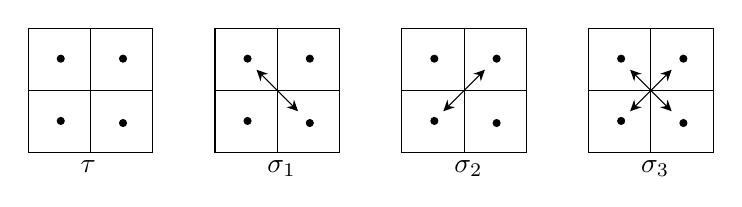
\begin{tikzpicture}[x=0.75pt,y=0.75pt,yscale=-1,xscale=1]
		%uncomment if require: \path (0,300); %set diagram left start at 0, and has height of 300
		
		%Shape: Square [id:dp32281460324226097] 
		\draw   (140,110) -- (200,110) -- (200,170) -- (140,170) -- cycle ;
		%Shape: Square [id:dp8196638610158489] 
		\draw   (140,140) -- (170,140) -- (170,170) -- (140,170) -- cycle ;
		%Shape: Square [id:dp5774035572053016] 
		\draw   (170,110) -- (200,110) -- (200,140) -- (170,140) -- cycle ;
		%Shape: Circle [id:dp09891447874029646] 
		\draw  [fill={rgb, 255:red, 0; green, 0; blue, 0 }  ,fill opacity=1 ] (154,154.67) .. controls (154,153.75) and (154.75,153) .. (155.67,153) .. controls (156.59,153) and (157.33,153.75) .. (157.33,154.67) .. controls (157.33,155.59) and (156.59,156.33) .. (155.67,156.33) .. controls (154.75,156.33) and (154,155.59) .. (154,154.67) -- cycle ;
		%Shape: Circle [id:dp22116361037170384] 
		\draw  [fill={rgb, 255:red, 0; green, 0; blue, 0 }  ,fill opacity=1 ] (154,124.67) .. controls (154,123.75) and (154.75,123) .. (155.67,123) .. controls (156.59,123) and (157.33,123.75) .. (157.33,124.67) .. controls (157.33,125.59) and (156.59,126.33) .. (155.67,126.33) .. controls (154.75,126.33) and (154,125.59) .. (154,124.67) -- cycle ;
		%Shape: Circle [id:dp9650296343672273] 
		\draw  [fill={rgb, 255:red, 0; green, 0; blue, 0 }  ,fill opacity=1 ] (184,124.67) .. controls (184,123.75) and (184.75,123) .. (185.67,123) .. controls (186.59,123) and (187.33,123.75) .. (187.33,124.67) .. controls (187.33,125.59) and (186.59,126.33) .. (185.67,126.33) .. controls (184.75,126.33) and (184,125.59) .. (184,124.67) -- cycle ;
		%Shape: Circle [id:dp04305617583331389] 
		\draw  [fill={rgb, 255:red, 0; green, 0; blue, 0 }  ,fill opacity=1 ] (184,155.67) .. controls (184,154.75) and (184.75,154) .. (185.67,154) .. controls (186.59,154) and (187.33,154.75) .. (187.33,155.67) .. controls (187.33,156.59) and (186.59,157.33) .. (185.67,157.33) .. controls (184.75,157.33) and (184,156.59) .. (184,155.67) -- cycle ;
		%Shape: Square [id:dp9546517027938655] 
		\draw   (230,110) -- (290,110) -- (290,170) -- (230,170) -- cycle ;
		%Shape: Square [id:dp9796040587153678] 
		\draw   (230,140) -- (260,140) -- (260,170) -- (230,170) -- cycle ;
		%Shape: Square [id:dp44002801088017396] 
		\draw   (260,110) -- (290,110) -- (290,140) -- (260,140) -- cycle ;
		%Shape: Circle [id:dp8334842171707744] 
		\draw  [fill={rgb, 255:red, 0; green, 0; blue, 0 }  ,fill opacity=1 ] (244,154.67) .. controls (244,153.75) and (244.75,153) .. (245.67,153) .. controls (246.59,153) and (247.33,153.75) .. (247.33,154.67) .. controls (247.33,155.59) and (246.59,156.33) .. (245.67,156.33) .. controls (244.75,156.33) and (244,155.59) .. (244,154.67) -- cycle ;
		%Shape: Circle [id:dp7038719736923629] 
		\draw  [fill={rgb, 255:red, 0; green, 0; blue, 0 }  ,fill opacity=1 ] (244,124.67) .. controls (244,123.75) and (244.75,123) .. (245.67,123) .. controls (246.59,123) and (247.33,123.75) .. (247.33,124.67) .. controls (247.33,125.59) and (246.59,126.33) .. (245.67,126.33) .. controls (244.75,126.33) and (244,125.59) .. (244,124.67) -- cycle ;
		%Shape: Circle [id:dp31839873684913567] 
		\draw  [fill={rgb, 255:red, 0; green, 0; blue, 0 }  ,fill opacity=1 ] (274,124.67) .. controls (274,123.75) and (274.75,123) .. (275.67,123) .. controls (276.59,123) and (277.33,123.75) .. (277.33,124.67) .. controls (277.33,125.59) and (276.59,126.33) .. (275.67,126.33) .. controls (274.75,126.33) and (274,125.59) .. (274,124.67) -- cycle ;
		%Shape: Circle [id:dp4037814749975406] 
		\draw  [fill={rgb, 255:red, 0; green, 0; blue, 0 }  ,fill opacity=1 ] (274,155.67) .. controls (274,154.75) and (274.75,154) .. (275.67,154) .. controls (276.59,154) and (277.33,154.75) .. (277.33,155.67) .. controls (277.33,156.59) and (276.59,157.33) .. (275.67,157.33) .. controls (274.75,157.33) and (274,156.59) .. (274,155.67) -- cycle ;
		%Shape: Square [id:dp21356453024304045] 
		\draw   (320,110) -- (380,110) -- (380,170) -- (320,170) -- cycle ;
		%Shape: Square [id:dp8300128863871687] 
		\draw   (320,140) -- (350,140) -- (350,170) -- (320,170) -- cycle ;
		%Shape: Square [id:dp3841760757181829] 
		\draw   (350,110) -- (380,110) -- (380,140) -- (350,140) -- cycle ;
		%Shape: Circle [id:dp06400640599899687] 
		\draw  [fill={rgb, 255:red, 0; green, 0; blue, 0 }  ,fill opacity=1 ] (334,154.67) .. controls (334,153.75) and (334.75,153) .. (335.67,153) .. controls (336.59,153) and (337.33,153.75) .. (337.33,154.67) .. controls (337.33,155.59) and (336.59,156.33) .. (335.67,156.33) .. controls (334.75,156.33) and (334,155.59) .. (334,154.67) -- cycle ;
		%Shape: Circle [id:dp4219802758838924] 
		\draw  [fill={rgb, 255:red, 0; green, 0; blue, 0 }  ,fill opacity=1 ] (334,124.67) .. controls (334,123.75) and (334.75,123) .. (335.67,123) .. controls (336.59,123) and (337.33,123.75) .. (337.33,124.67) .. controls (337.33,125.59) and (336.59,126.33) .. (335.67,126.33) .. controls (334.75,126.33) and (334,125.59) .. (334,124.67) -- cycle ;
		%Shape: Circle [id:dp12957899145925378] 
		\draw  [fill={rgb, 255:red, 0; green, 0; blue, 0 }  ,fill opacity=1 ] (364,124.67) .. controls (364,123.75) and (364.75,123) .. (365.67,123) .. controls (366.59,123) and (367.33,123.75) .. (367.33,124.67) .. controls (367.33,125.59) and (366.59,126.33) .. (365.67,126.33) .. controls (364.75,126.33) and (364,125.59) .. (364,124.67) -- cycle ;
		%Shape: Circle [id:dp09206954889493102] 
		\draw  [fill={rgb, 255:red, 0; green, 0; blue, 0 }  ,fill opacity=1 ] (364,155.67) .. controls (364,154.75) and (364.75,154) .. (365.67,154) .. controls (366.59,154) and (367.33,154.75) .. (367.33,155.67) .. controls (367.33,156.59) and (366.59,157.33) .. (365.67,157.33) .. controls (364.75,157.33) and (364,156.59) .. (364,155.67) -- cycle ;
		%Shape: Square [id:dp38707064557107107] 
		\draw   (410,110) -- (470,110) -- (470,170) -- (410,170) -- cycle ;
		%Shape: Square [id:dp016467202872691322] 
		\draw   (410,140) -- (440,140) -- (440,170) -- (410,170) -- cycle ;
		%Shape: Square [id:dp24812893227031285] 
		\draw   (440,110) -- (470,110) -- (470,140) -- (440,140) -- cycle ;
		%Shape: Circle [id:dp18320251504349438] 
		\draw  [fill={rgb, 255:red, 0; green, 0; blue, 0 }  ,fill opacity=1 ] (424,154.67) .. controls (424,153.75) and (424.75,153) .. (425.67,153) .. controls (426.59,153) and (427.33,153.75) .. (427.33,154.67) .. controls (427.33,155.59) and (426.59,156.33) .. (425.67,156.33) .. controls (424.75,156.33) and (424,155.59) .. (424,154.67) -- cycle ;
		%Shape: Circle [id:dp1417318830130958] 
		\draw  [fill={rgb, 255:red, 0; green, 0; blue, 0 }  ,fill opacity=1 ] (424,124.67) .. controls (424,123.75) and (424.75,123) .. (425.67,123) .. controls (426.59,123) and (427.33,123.75) .. (427.33,124.67) .. controls (427.33,125.59) and (426.59,126.33) .. (425.67,126.33) .. controls (424.75,126.33) and (424,125.59) .. (424,124.67) -- cycle ;
		%Shape: Circle [id:dp5953928915650424] 
		\draw  [fill={rgb, 255:red, 0; green, 0; blue, 0 }  ,fill opacity=1 ] (454,124.67) .. controls (454,123.75) and (454.75,123) .. (455.67,123) .. controls (456.59,123) and (457.33,123.75) .. (457.33,124.67) .. controls (457.33,125.59) and (456.59,126.33) .. (455.67,126.33) .. controls (454.75,126.33) and (454,125.59) .. (454,124.67) -- cycle ;
		%Shape: Circle [id:dp5197879342370941] 
		\draw  [fill={rgb, 255:red, 0; green, 0; blue, 0 }  ,fill opacity=1 ] (454,155.67) .. controls (454,154.75) and (454.75,154) .. (455.67,154) .. controls (456.59,154) and (457.33,154.75) .. (457.33,155.67) .. controls (457.33,156.59) and (456.59,157.33) .. (455.67,157.33) .. controls (454.75,157.33) and (454,156.59) .. (454,155.67) -- cycle ;
		%Straight Lines [id:da1668296738798587] 
		\draw    (252.12,132.12) -- (267.88,147.88) ;
		\draw [shift={(270,150)}, rotate = 225] [fill={rgb, 255:red, 0; green, 0; blue, 0 }  ][line width=0.08]  [draw opacity=0] (5.36,-2.57) -- (0,0) -- (5.36,2.57) -- (3.56,0) -- cycle    ;
		\draw [shift={(250,130)}, rotate = 45] [fill={rgb, 255:red, 0; green, 0; blue, 0 }  ][line width=0.08]  [draw opacity=0] (5.36,-2.57) -- (0,0) -- (5.36,2.57) -- (3.56,0) -- cycle    ;
		%Straight Lines [id:da6153426025313546] 
		\draw    (357.88,132.12) -- (342.12,147.88) ;
		\draw [shift={(340,150)}, rotate = 315] [fill={rgb, 255:red, 0; green, 0; blue, 0 }  ][line width=0.08]  [draw opacity=0] (5.36,-2.57) -- (0,0) -- (5.36,2.57) -- (3.56,0) -- cycle    ;
		\draw [shift={(360,130)}, rotate = 135] [fill={rgb, 255:red, 0; green, 0; blue, 0 }  ][line width=0.08]  [draw opacity=0] (5.36,-2.57) -- (0,0) -- (5.36,2.57) -- (3.56,0) -- cycle    ;
		%Straight Lines [id:da47301045731826874] 
		\draw    (447.88,132.12) -- (432.12,147.88) ;
		\draw [shift={(430,150)}, rotate = 315] [fill={rgb, 255:red, 0; green, 0; blue, 0 }  ][line width=0.08]  [draw opacity=0] (5.36,-2.57) -- (0,0) -- (5.36,2.57) -- (3.56,0) -- cycle    ;
		\draw [shift={(450,130)}, rotate = 135] [fill={rgb, 255:red, 0; green, 0; blue, 0 }  ][line width=0.08]  [draw opacity=0] (5.36,-2.57) -- (0,0) -- (5.36,2.57) -- (3.56,0) -- cycle    ;
		%Straight Lines [id:da5852456111119229] 
		\draw    (432.12,132.12) -- (447.88,147.88) ;
		\draw [shift={(450,150)}, rotate = 225] [fill={rgb, 255:red, 0; green, 0; blue, 0 }  ][line width=0.08]  [draw opacity=0] (5.36,-2.57) -- (0,0) -- (5.36,2.57) -- (3.56,0) -- cycle    ;
		\draw [shift={(430,130)}, rotate = 45] [fill={rgb, 255:red, 0; green, 0; blue, 0 }  ][line width=0.08]  [draw opacity=0] (5.36,-2.57) -- (0,0) -- (5.36,2.57) -- (3.56,0) -- cycle    ;
		
		% Text Node
		\draw (164,172.4) node [anchor=north west][inner sep=0.75pt]    {$\tau $};
		% Text Node
		\draw (254,172.4) node [anchor=north west][inner sep=0.75pt]    {$\sigma _{1}$};
		% Text Node
		\draw (344,172.4) node [anchor=north west][inner sep=0.75pt]    {$\sigma _{2}$};
		% Text Node
		\draw (434,172.4) node [anchor=north west][inner sep=0.75pt]    {$\sigma _{3}$};
		
		
	\end{tikzpicture}
\end{figure} 
\begin{conjecture}
	There are no other choices for $ \tau, \sigma_1,\sigma_2, \sigma_3 $ that generates a self similar pattern.
\end{conjecture}
\begin{remark}
	My intuition about the truth of the conjecture above starts from the fact are no other two permutations except for swapping the elements on the main diagonal and non-main diagonal of a $ 2\times 2 $ matrix that has $ 2 $ fixed points. 
\end{remark}
\begin{figure}[h!]
	\centering
	\includegraphics[width=0.8\linewidth]{code/high_resolution_plot}
\end{figure}
\FloatBarrier
\noindent End.




\end{document}
